\documentclass[conference]{IEEEtran}

%\IEEEoverridecommandlockouts
%\IEEEoverridecommandlockouts
% The preceding line is only needed to identify funding in the first footnote.
% If that is unneeded, please comment it out.

\usepackage{cite}
\usepackage{amsmath,amssymb,amsfonts}
\usepackage{diffcoeff}
\usepackage{isomath}
\usepackage{siunitx}
\usepackage{graphicx}
\usepackage{textcomp}
\usepackage{makecell}
\catcode`\_=12
\usepackage{xcolor}
\usepackage{booktabs}
\newlength\imagewidth
\newlength\imagescale
\usepackage[nonumberlist,acronym,nomain]{glossaries}
\usepackage{cleveref}
\usepackage{float}
\sisetup{table-format=1.3}
\usepackage{algorithm}
\usepackage{algpseudocode}
\usepackage{pgf}
\usepackage{lmodern}
\catcode`\_=12
\usepackage{pgfplots}
\pgfplotsset{compat=1.18}
\pgfplotsset{
every axis/.append style={
title style={font=\bfseries\normalsize},
label style={font=\normalsize},
tick label style={font=\small},
legend style={font=\footnotesize}
}
}
\usepackage{tikz}
\usepackage[T1]{fontenc}
\usepackage[utf8]{inputenc}
\usepackage{url}
\setlength{\columnsep}{0.25in}

% Shared graphs folder
\newcommand{\graphpath}{../E_P_E_of_a_Multi_Vendor_P_5G_Testbed/graphs}

\DeclareMathOperator{\csch}{csch}
\newcommand{\e}{\ensuremath{\text{e}}}
\newcommand{\infint}{\ensuremath{\int_{\infty}^{\infty}}}
\newcommand{\hpoly}[2][n]{\ensuremath{\exp\left\{-\frac{{#2}^2}{2}\right\} H_{#1}\left(#2\right)}}
\newcommand{\hpolye}[2][n]{\ensuremath{\e^{-\frac{{#2}^2}{2}} H_{#1}\left(#2\right)}}
\newcommand{\hpolyp}[2][n]{\ensuremath{\exp\left\{-\frac{\left(#2\right)^2}{2}\right\} H_{#1}\left(#2\right)}}
\newcommand{\F}{\ensuremath{\mathcal{F}}}
\newcommand{\paperTwopdfpath}{../csvandexcelfiles/paper2/pdfGraphs}

\def\BibTeX{{\rm B\kern-.05em{\sc i\kern-.025em b}\kern-.08em
T\kern-.1667em\lower.7ex\hbox{E}\kern-.125emX}}

\loadglsentries{acronyms.tex}

\pgfplotsset{
  every axis title/.append style={font=\bfseries\large},
  every axis x label/.append style={font=\normalsize},
  every axis y label/.append style={font=\normalsize},
  every tick label/.append style={font=\small},
  every axis legend/.append style={font=\scriptsize}
}


\begin{document}

\title{From Simulation to Real-World Validation: Assessing the Experimental Maturity of DECT-2020 NR Research}

\author{\IEEEauthorblockN{Ashuqullah Alizai}
\IEEEauthorblockA{\textit{Aalen University of Applied Sciences} \\
Aalen, Germany \\
ashuqullah.alizai@hs-aalen.de\\ ORCID 0000-0002-7625-2330}
\and
\IEEEauthorblockN{Mohammad Reza Mousavi}
\IEEEauthorblockA{\textit{Aalen University of Applied Sciences} \\
Aalen, Germany \\
mohammad.mousavi@hs-aalen.de\\ ORCID 0000-0003-2521-2651}
\and
\IEEEauthorblockN{Daryoosh Mansory}
\IEEEauthorblockA{\textit{Herat University} \\
Herat, Afghanistan \\
d.mansoory786@hu.edu.af\\ ORCID 0009-0001-6085-4580}

\and
\IEEEauthorblockN{Milad Goodarzi}
\IEEEauthorblockA{\textit{Aalen University of Applied Sciences} \\
Aalen, Germany \\
milad.goodarzi@hs-aalen.de\\ ORCID 0000-0000-0000-0000}

\and
\IEEEauthorblockN{Stephan Ludwig}
\IEEEauthorblockA{\textit{Aalen University of Applied Sciences} \\
Aalen, Germany \\
stephan.ludwig@hs-aalen.de\\ORCID 0000-0002-0233-1706}
}

\maketitle

\begin{abstract}
\gls{dectnr} is a non-cellular \gls{imt2020} radio technology
supporting decentralized and infrastructure-light wireless
communication. Although research has progressed from analytical and
simulation-based studies toward practical implementations, its
experimental maturity has not been systematically assessed.

This paper analyzes the experimental maturity of \gls{dectnr} based
on 51 primary studies published between 2020 and July 2026.
Simulation remains the dominant evaluation methodology, appearing in
32 studies, while 16 studies employ experimental or testbed-based
evaluation. Hardware prototypes are reported in 16 studies and
commercial-device evaluations in 11, whereas only five studies report
field trials and three report industrial measurements. A cross-analysis
of technical areas and validation approaches reveals uneven maturity:
\gls{phy} research shows comparatively strong hardware and practical
validation, while routing and mesh networking remain predominantly
simulation-based and scheduling and resource allocation have limited
experimental evidence. Based on these findings, a five-level
experimental-maturity framework is proposed, and large-scale physical
testbeds, application-oriented validation, long-duration measurements,
and reproducible benchmarking are identified as key priorities for
future \gls{dectnr} research.
\end{abstract}

\section{Introduction}
\label{sec:introduction}

Next-generation wireless networks increasingly support \gls{iot} and
industrial applications with heterogeneous requirements for latency,
reliability, energy efficiency, scalability, coverage, mobility, and
predictability
\cite{sisinniIndustrialInternetThings2018,
wollschlaegerFutureIndustrialCommunication2017a}. Within this
landscape, \gls{dectnr} has emerged as a non-cellular \gls{imt2020}
radio technology designed for decentralized and infrastructure-light
wireless communication. Its flexible device roles, autonomous
radio-resource operation, and support for direct and multi-hop
communication make it particularly relevant to \gls{iot} and
\gls{iiot} deployments requiring local network ownership, dense
connectivity, and flexible network topologies
\cite{itur_m2150,
kovalchukovDECT2020NewRadio2022,
perez-guiraoDECTNRUnveiling2022}.

Since its introduction, research on \gls{dectnr} has expanded
substantially. Early work concentrated primarily on \gls{imt2020}
candidate-technology assessment, link-level performance, and
compliance with communication requirements
\cite{pennerURLLCPerformanceEvaluation2021,
maliatsosEvaluationIMT2020Candidate2022a,
smidaETSIDECT2020Component2023}. Subsequent research has addressed a
broader range of topics, including \gls{phy} and \gls{mac}
mechanisms, multi-hop and mesh networking, routing, resource
management, reliability, energy efficiency, positioning,
coexistence, and application-oriented implementations. At the same
time, evaluation has begun to progress beyond analytical and
simulation-based investigation toward \gls{sdr} and \gls{fpga}
implementations, commercial devices, hardware prototypes, field
trials, and industrial measurements
\cite{fagerholmFPGAbasedDECT2020New2024,
wassmannPerformanceDECT2020NR2024,
bandaraExperimentalValidationAnalysis2025,
grafWhatExpectWhen2026}.

This progression from theoretical investigation toward physical
validation is particularly important for assessing the practical
capabilities of \gls{dectnr}. Analytical models and simulation provide
essential means for investigating protocol behavior, scalability, and
performance under controlled and reproducible assumptions. However,
they cannot fully capture implementation- and deployment-dependent
effects such as transceiver turnaround, processing overhead,
synchronization behavior, practical propagation and interference,
hardware energy consumption, radio-state transitions, and
implementation-specific protocol interactions. These effects become
increasingly important when evaluating multi-device, multi-hop, and
latency- or reliability-sensitive communication under realistic
operating conditions.

Despite the increasing number of experimental studies, the extent to
which \gls{dectnr} research has progressed toward physical,
integrated-system, and real-world validation has not been
systematically characterized across technical areas. Existing work
provides evidence for individual mechanisms and use cases, but does
not reveal whether experimental maturity has developed uniformly
across the research landscape. Consequently, it remains unclear which
technical areas are supported by substantial hardware and real-world
evidence, which remain predominantly dependent on analytical or
simulation-based evaluation, and where the principal experimental
validation gaps persist.

To address this gap, this paper performs a focused secondary analysis
of a systematically established corpus of 51 \gls{dectnr} studies
published between 2020 and July 2026. Rather than providing another
general technical survey, the study examines how the available
evidence progresses from analytical feasibility and simulation toward
prototype, integrated-system, and industrial validation. The main
contributions of this paper are:

\begin{itemize}
    \item a quantitative mapping of evaluation methodologies and
    validation approaches across a systematically established corpus
    of 51 \gls{dectnr} studies;

    \item a cross-analysis of experimental maturity across major
    technical research areas, identifying where research volume is
    supported by physical and real-world evidence and where validation
    remains predominantly analytical or simulation-based; and

    \item a five-level experimental-maturity framework relating
    analytical feasibility, simulation validation, prototype
    validation, integrated-system validation, and industrial
    integration, together with research priorities for reproducible,
    application-oriented, and real-world \gls{dectnr} validation.
\end{itemize}

The remainder of this paper is organized as follows.
Section~\ref{sec:methodology} describes the systematic mapping
methodology. Section~\ref{sec:maturity} analyzes the evaluation
landscape and experimental maturity across technical areas.
Section~\ref{sec:framework} introduces the proposed maturity
framework, and Section~\ref{sec:conclusion} concludes the paper.


\section{Systematic Mapping Methodology}
\label{sec:methodology}

This study analyzes the experimental maturity of \gls{dectnr} using
a \gls{prisma}-based \gls{slr} corpus covering publications from
January 2020 to July 2026. The underlying review process was designed
to identify, screen, classify, and synthesize research addressing the
architecture, protocols, implementation, and performance evaluation of
\gls{dectnr}. Normative \gls{etsi} specifications and relevant
\gls{itur} recommendations were analyzed separately to provide
technical and standardization context and were not counted as primary
research studies in the quantitative analysis.

The experimental-maturity analysis addresses the following research
questions:

\begin{itemize}
    \item[\textbf{RQ1}] How has \gls{dectnr} research progressed from
    analytical and simulation-based evaluation toward experimental and
    real-world validation?

    \item[\textbf{RQ2}] Which technical areas have accumulated
    experimental evidence, and which remain predominantly dependent on
    simulation or analytical evaluation?

    \item[\textbf{RQ3}] Which experimental and methodological gaps must
    be addressed to enable reproducible and application-oriented
    validation?
\end{itemize}

\subsection{Corpus and Study Selection}
\label{subsec:corpus}

IEEE Xplore, Scopus, ACM Digital Library, SpringerLink, and
ScienceDirect were searched for relevant publications. Google Scholar
was used as a complementary source for backward and forward
snowballing rather than as an additional primary database. The search
covered publications from January 2020 to July 2026 and used the
following Boolean query:

\begin{quote}
\footnotesize
(\texttt{"DECT-2020 NR"} OR \texttt{"DECT NR+"} OR
\texttt{"DECT-2020 New Radio"} OR \texttt{"DECT NR"} OR
\texttt{"DECT New Radio"}) AND
(\texttt{architecture} OR \texttt{protocol} OR \texttt{PHY} OR
\texttt{"physical layer"} OR \texttt{MAC} OR
\texttt{"medium access control"} OR \texttt{implementation} OR
\texttt{experimental} OR \texttt{testbed} OR \texttt{prototype} OR
\texttt{performance} OR \texttt{evaluation} OR \texttt{measurement} OR
\texttt{industrial} OR \texttt{IoT} OR \texttt{URLLC} OR
\texttt{reliability})
\end{quote}

Studies were considered eligible when they investigated
\gls{dectnr} as a primary technology and reported a technical,
methodological, implementation-oriented, or performance-related
contribution. Publications not primarily concerned with
\gls{dectnr}, duplicate records, and documents without sufficient
technical relevance to the research questions were excluded.
Normative standards and recommendations were retained separately as
contextual sources and were excluded from the primary-study count.

The primary database searches identified 107 records: 42 from IEEE
Xplore, 44 from Scopus, one from ACM Digital Library, 15 from
SpringerLink, and five from ScienceDirect. An additional 226 records
were examined through complementary snowballing. After duplicate
handling, title and abstract screening, retrieval, and full-text
eligibility assessment, 51 primary studies were retained for the
systematic mapping. The complete study-selection process is shown in
Fig.~\ref{fig:prisma}.

\begin{figure}[!t]
    \centering
    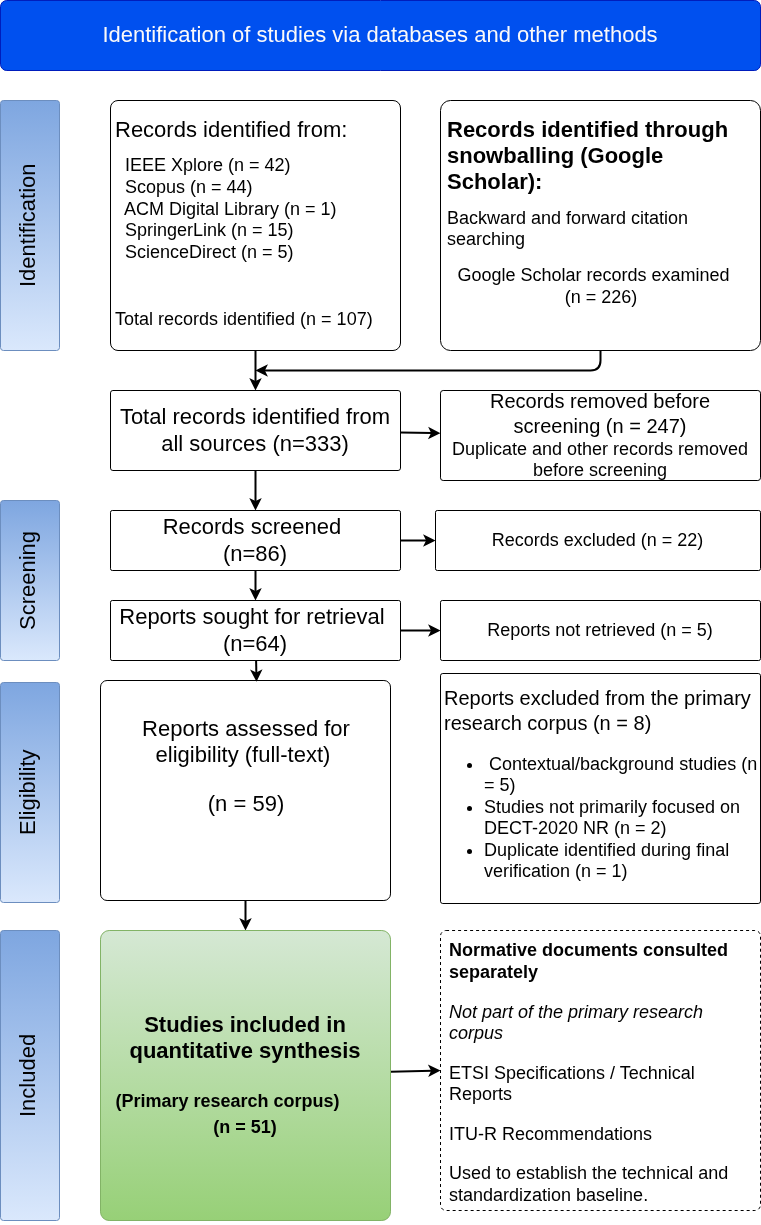
\includegraphics[width=0.85\columnwidth]
    {figures/PRISMA_Result.png}
    \caption{\gls{prisma} flow diagram of the study-selection process.}
    \label{fig:prisma}
\end{figure}

\subsection{Experimental-Maturity Coding}
\label{subsec:maturity_coding}

Each of the 51 primary studies was systematically coded along five
dimensions: technical topic, evaluation methodology, validation
approach, implementation platform, and reported \glspl{kpi}. The
coding scheme was multi-label, allowing a study to contribute to more
than one technical area, methodology, validation approach, platform,
or performance metric when supported by the reported evaluation.

Technical topics included \gls{phy}, \gls{mac}, routing and mesh
networking, scheduling and resource allocation, energy efficiency,
positioning, security and multi-RAT integration, coexistence and
regulation, \gls{urllc}, and \gls{mmtc}. Evaluation methodologies
were coded as simulation, analytical/modeling,
experimental/testbed, or survey/overview according to the methods
reported by each study.

For the experimental-maturity analysis, validation evidence was
grouped into five categories. \emph{Analytical} evidence comprises
mathematical and model-based investigation, while \emph{simulation}
captures software-based numerical or event-driven evaluation.
\emph{Prototype/hardware} evidence combines hardware prototypes and
\gls{sdr}/over-the-air implementations. \emph{Commercial
device/testbed} identifies evaluations using commercial devices, and
\emph{field/industrial} combines field trials and industrial
measurements. These categories were cross-analyzed with the technical
topics to determine where research has progressed toward physical and
real-world validation.

Because both technical topics and validation approaches are
multi-label, category totals are not mutually exclusive and therefore
do not sum to the 51 included studies. This coding strategy enables
the analysis to distinguish research volume from experimental
maturity: a frequently investigated technical area may still have
limited prototype, testbed, or field-level evidence.
\section{Experimental Maturity of DECT-2020 NR Research}
\label{sec:maturity}

\subsection{Evaluation Landscape}
\label{subsec:evaluation_landscape}

The 51-study corpus shows substantial recent growth, with 38 studies
(approximately 75\%) published between 2024 and July 2026. Simulation
remains the dominant evaluation methodology, appearing in 32 studies,
followed by analytical/modeling approaches in 23 studies and
experimental/testbed evaluation in 16. Nine studies additionally
employ survey or overview methodologies. Because these categories are
multi-label, individual studies may employ multiple evaluation
approaches.

Figure~\ref{fig:evaluation_methods} shows that, despite increasing
experimental activity, analytical and simulation-based evaluation
still constitutes a substantial part of the evidence base. The
presence of experimental/testbed evaluation in 16 studies nevertheless
indicates a visible transition from feasibility-oriented investigation
toward physical implementation and practical validation, although this
transition is uneven across technical research areas.

\begin{figure}[!t]
    \centering
    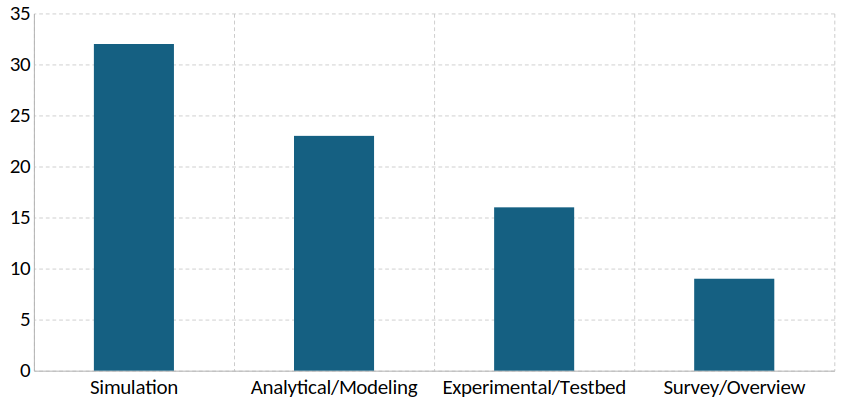
\includegraphics[width=\columnwidth]{figures/fig5.png}
    \caption{Evaluation methodologies employed across the 51 included
    studies (multi-label).}
    \label{fig:evaluation_methods}
\end{figure}


\subsection{Experimental Maturity Across Technical Areas}
\label{subsec:maturity_matrix}

Table~\ref{tab:maturity_matrix} cross-analyzes the major technical
areas with their validation approaches. Prototype/hardware evidence
combines hardware prototypes and \gls{sdr}/over-the-air validation,
while field/industrial evidence combines field trials and industrial
measurements. Because both technical areas and validation approaches
are multi-label, the values should be interpreted as overlapping
evidence rather than mutually exclusive study counts.

\begin{table*}[!t]
\centering
\caption{Experimental maturity across major \gls{dectnr} research
areas in the 51-study corpus. Categories are multi-label; therefore,
individual studies may contribute to multiple research areas and
validation approaches.}
\label{tab:maturity_matrix}
\resizebox{\textwidth}{!}{%
\begin{tabular}{lrrrrrr}
\toprule
\textbf{Research Area} &
\textbf{Studies} &
\textbf{Analytical} &
\textbf{Simulation} &
\textbf{Prototype/Hardware} &
\textbf{Commercial Device/Testbed} &
\textbf{Field/Industrial} \\
\midrule
\gls{phy}                         & 22 & 10 & 10 & 11 & 8 & 5 \\
\gls{mac}                         & 22 & 11 & 16 &  4 & 2 & 0 \\
Routing/Mesh                      & 23 & 12 & 17 &  3 & 1 & 1 \\
Scheduling/Resources              &  4 &  3 &  3 &  1 & 1 & 0 \\
Energy                            &  8 &  2 &  3 &  5 & 4 & 2 \\
Positioning                       &  6 &  6 &  4 &  2 & 2 & 1 \\
Security/Multi-RAT                &  3 &  0 &  0 &  3 & 0 & 0 \\
Coexistence/Regulation            &  2 &  0 &  2 &  0 & 0 & 0 \\
\gls{urllc}                       &  9 &  3 &  8 &  1 & 1 & 0 \\
\gls{mmtc}                        &  5 &  2 &  5 &  0 & 0 & 0 \\
\bottomrule
\end{tabular}}
\end{table*}

The results reveal substantial differences between research volume
and experimental maturity. Routing/mesh constitutes the largest
technical cluster, yet 17 of its 23 studies employ simulation and
only three provide prototype/hardware evidence. In contrast,
\gls{phy} research shows the strongest progression toward physical
validation, with 11 of 22 studies reporting prototype/hardware
evidence, eight involving commercial-device/testbed validation, and
five reaching field/industrial evaluation. \gls{mac}, \gls{urllc},
and \gls{mmtc} remain considerably more simulation-oriented.

A notable pattern is that research volume and experimental maturity
do not evolve proportionally. Routing/mesh and \gls{mac} are among
the most frequently investigated areas, yet their evidence remains
dominated by simulation. In contrast, energy research has a smaller
publication base but a comparatively high proportion of hardware and
commercial-device validation. This difference may partly reflect the
practical complexity of experimental validation. Device- and
link-level behavior can often be investigated using relatively small
setups, whereas routing, scheduling, and multi-hop mechanisms require
larger synchronized deployments, controlled multi-device traffic, and
repeatable network-level experiments. Research volume alone is
therefore not a sufficient indicator of practical validation maturity.


\subsection{PHY and MAC}
\label{subsec:phy_mac}

Early \gls{phy} research concentrated on candidate-technology
assessment, \gls{imt2020} compliance, link-level behavior, modulation
and coding, and system-level performance
\cite{dhanwaniAssessmentCandidateTechnology2020,
pennerLinkLevelPerformanceEvaluation2021,
pennerURLLCPerformanceEvaluation2021,
singhwiDECT2020NewRadio2021,
maliatsosEvaluationIMT2020Candidate2022a,
smidaETSIDECT2020Component2023}.
Subsequent studies extended this evidence toward channel estimation,
\gls{noma}, propagation and range measurements, industrial-channel
characterization, \gls{fpga}-oriented implementation, and
commercial-hardware evaluation
\cite{kizilirmakExaminationPHYLayer2024,
llagunoPhysicalLayerPerformance2024,
fagerholmFPGAbasedDECT2020New2024,
wassmannPerformanceDECT2020NR2024,
haqueDECT2020NRLink2025,
liuDataAidedChannelEstimation2025,
soniLinkLevelAssessmentNOMA2023,
bandaraExperimentalValidationAnalysis2025,
grafParetoOptimalityApproach2026a,
grafWhatExpectWhen2026}.

The maturity profile of \gls{mac} research is less experimental.
Although \gls{mac} aspects appear in 22 studies, 16 employ simulation
and only four provide prototype/hardware evidence. Existing work
addresses outage reduction, relaying, random access, coexistence,
reliability, and multi-hop access
\cite{ahmadMACProtocolReducing2024,
ahmadMACLayerProtocolUltraReliable2025,
gaidamakaOptimizingDelaysRandom2025,
samuylovPerformanceAssessmentDECT20202023,
samuylovPerformanceMACLayer2024a,
samuylovEmpoweringNearURLLCIoT2025}.
Measurement-driven results further show that hardware effects such as
RX--TX turnaround and single-transceiver operation can directly affect
UL/DL scheduling latency
\cite{alizaiMeasurementDrivenLatencyAnalysis2026}, emphasizing the
need for physical multi-device validation.

This distinction is particularly important for \gls{mac} evaluation.
Simulation can characterize protocol logic, channel access, and
resource-allocation behavior under controlled assumptions, but
practical performance is additionally influenced by
implementation-dependent effects. Processing delays, synchronization,
radio-state transitions, channel sensing, and transceiver turnaround
can affect application-visible latency and reliability. Physical
validation is therefore particularly important when assessing
\gls{urllc}-oriented or deterministic communication mechanisms whose
performance depends on interactions between protocol operation and
hardware behavior.


\subsection{Routing, Mesh, and Resource Allocation}
\label{subsec:routing_resources}

Routing and mesh networking constitute the largest technical cluster,
with 23 studies addressing flooding, source routing, relay assignment,
deep mesh topologies, reliability-oriented path selection, and
multi-hop forwarding
\cite{soniPerformanceMultihopAssisted2021,
kovalchukovDECT2020NewRadio2022,
biswasReliableLowLatencyCommunications2024,
fuhrlingRobustRoutingProtocol2025b,
asifURLLCBasedMultiHopCommunication2025,
glazkovImprovingNearURLLCServices2025,
samuylovPerformanceDECT2020NR2025,
alamDLRoutingPerformance2026a,
morozovaComparisonTwoModels2026a,
nikolaevModelingDECT2020Tandem2026,
rauwolfTopologyAwareDeepReinforcement2026a}.

Despite this research volume, 17 studies rely on simulation, while
only three provide prototype/hardware evidence and one reaches
field/industrial validation. Large-scale physical mesh validation
therefore remains a major gap. This is particularly relevant because
behavior observed in simulated multi-hop networks may become more
difficult to reproduce as physical network depth and device density
increase. Contention, accumulated forwarding delay, interference,
route instability, synchronization effects, and concurrent traffic
may interact across multiple hops. Larger physical topologies are
therefore needed to determine whether the scalability demonstrated in
simulation translates into predictable end-to-end performance under
implementation and deployment constraints.

Scheduling and resource allocation form a much smaller evidence base,
appearing in only four studies
\cite{samuylovPerformanceAssessmentDECT20202023,
binasifIRSAssistedDECT2020NR2025,
rauwolfTopologyAwareDeepReinforcement2026a,
grafParetoOptimalityApproach2026a}.
Only one provides prototype/hardware and commercial-device evidence.
Together with measurement-driven observations of practical
transceiver constraints
\cite{alizaiMeasurementDrivenLatencyAnalysis2026}, this indicates a
need for application-oriented scheduling evaluated on physical
multi-device systems.

The limited experimental evidence in this area is particularly
relevant to industrial communication because scheduling and resource
allocation connect lower-layer radio capabilities with
application-visible performance. Decisions concerning resource
assignment, transmission opportunities, retransmissions, and UL/DL
operation can directly influence latency, reliability, throughput,
and energy consumption. Consequently, evaluating these mechanisms
under heterogeneous traffic and multiple simultaneously active
devices represents an important step toward application-oriented
\gls{dectnr} validation.


\subsection{Application-Oriented and Emerging Areas}
\label{subsec:emerging_areas}

Energy-related research exhibits comparatively strong experimental
maturity: five of eight studies contain prototype/hardware evidence
and four use commercial-device validation. Existing work addresses
modem energy consumption, multi-hop energy trade-offs, router
rotation, and energy-aware operation
\cite{nihtilaEnergyConsumptionDECT20202022,
nihtilaEnergySavingRouter2022,
piresDECT2020NREnergy2026b,
grafWhatExpectWhen2026,
bandaraExperimentalValidationAnalysis2025}.
Positioning combines analytical and simulation-based investigations
with a smaller practical evidence base
\cite{saikkoPositioningDECT2020NR2024,
saikkoPositioningTrackingDECT20202025,
haqueDECT2020NRLink2025,
grafWhatExpectWhen2026}.

Multi-RAT integration forms a small but experimentally oriented
cluster, particularly through DECT/Wi-Fi integration and unified
radio-access implementations
\cite{dangEWDCIntegratingDECT20202025a,
dangUniRATUnifiedDECT20202026}.
Professional-audio implementations provide additional practical
evidence for application-oriented validation
\cite{durreDECT2020NRProfessional2024}.
In contrast, coexistence/regulatory studies remain predominantly
simulation-oriented
\cite{samuylovPerformanceAssessmentDECT20202023,
montalvoDECTEvolutionMeeting2024}.

The broader application landscape includes professional audio,
tactile communication, backscatter-assisted communication, and
LPWAN-oriented comparisons
\cite{poetsDECTNRNew2024,
poetsProfessionalNetworkedAudio2025,
mudriievskyiCHEAP5GDECT2024a,
liaoDataAssistedBackscatter2025,
leugnerAlternativeSubGHzLPWAN2025a,
jahangirAnalysisPerformanceDECT2024}.
These studies demonstrate the breadth of potential \gls{dectnr}
applications and deployment scenarios, but the available evidence
remains fragmented across application types, hardware platforms, and
experimental configurations. Broader application-oriented evaluation
is therefore needed to determine how technical mechanisms behave
under traffic patterns and operational requirements representative of
different industrial and \gls{iot} use cases.


\subsection{Experimental Platforms and Performance Evidence}
\label{subsec:platforms_metrics}

The transition toward physical validation is reflected in the
experimental platforms: 16 studies report hardware prototypes, 11
use commercial devices, five report field trials, and three include
industrial measurements. Nordic nRF91-series devices are the most
frequently identified commercial hardware platform, while other
studies employ \gls{sdr}, \gls{usrp}, GNU Radio, MATLAB, Zephyr, and
\gls{fpga}-oriented implementations.

Performance evaluation remains concentrated on packet error or loss,
reported in 40 studies, followed by energy/power in 22, latency in 15,
and reliability/outage in 15. Throughput appears in only five studies,
while application-level indicators such as fairness, \gls{aoi},
localization error, connection density, and spectral efficiency are
considerably less frequent. This distribution indicates that future
industrial validation should increasingly consider multiple
performance dimensions jointly, including latency, reliability,
throughput, jitter, energy consumption, mobility, and network
lifetime, rather than relying primarily on isolated average
\glspl{kpi}.

A further challenge is the heterogeneity of experimental setups.
Existing studies differ in hardware platforms, network size, topology,
traffic generation, radio configuration, propagation environment,
software and firmware implementation, and measurement duration. Such
diversity demonstrates the breadth of possible \gls{dectnr}
applications, but it also limits direct comparison across studies.
More consistent reporting of network configurations, traffic
characteristics, radio parameters, software and firmware versions,
measurement procedures, and statistical summaries would improve
reproducibility and enable more meaningful cross-study benchmarking.


\subsection{Cross-Layer Experimental Validation Gaps}
\label{subsec:validation_gaps}

The preceding results indicate that the remaining experimental
challenges are increasingly cross-layer rather than confined to
individual protocol mechanisms. Industrial communication performance
emerges from interactions among the \gls{phy}, \gls{mac}, routing,
scheduling, hardware behavior, traffic characteristics, and
application requirements. Consequently, successful validation of an
individual mechanism does not necessarily demonstrate predictable
end-to-end behavior in an integrated system.

A first gap concerns \emph{experimental scale}. Routing, mesh
networking, \gls{mmtc}, and resource-allocation studies frequently
target network sizes and traffic conditions that have not yet been
reproduced on comparably large physical testbeds. Increasing device
density and network depth introduces concurrent channel access,
interference, accumulated forwarding delay, synchronization effects,
route changes, and contention among heterogeneous traffic flows.
Large-scale multi-device experiments are therefore needed to
determine whether scalability demonstrated analytically or through
simulation persists under physical implementation constraints.

A second gap concerns \emph{cross-layer and application-oriented
evaluation}. Industrial applications may simultaneously impose
requirements on latency, reliability, throughput, energy consumption,
and communication predictability, whereas these properties are often
evaluated separately. Experimental campaigns should increasingly
combine heterogeneous traffic classes and examine how channel
conditions, \gls{mac} operation, scheduling, retransmissions, routing,
and hardware constraints jointly affect application-visible
performance. For latency- and reliability-sensitive communication,
distribution tails, failure events, and temporal variability are
particularly important alongside average \glspl{kpi}.

A third gap concerns \emph{reproducibility and comparability}.
Differences in hardware, firmware, network size, topology, traffic
generation, radio configuration, propagation environment, and
measurement duration make direct cross-study comparison difficult.
Reproducible evaluation therefore requires more consistent reporting
of experimental configurations, software and firmware versions,
traffic characteristics, measurement procedures, and statistical
distributions.

Together, these gaps indicate that experimental maturity should not
be judged solely by the presence of a hardware implementation.
Progress toward practical maturity increasingly requires larger
physical systems, cross-layer evaluation, realistic
application-oriented traffic, and repeatable integrated-system and
industrial experiments. These observations motivate the
experimental-maturity framework introduced in
Section~\ref{sec:framework}.
\section{Experimental-Maturity Framework}
\label{sec:framework}

The results in Table~\ref{tab:maturity_matrix} demonstrate that
\gls{dectnr} research progresses unevenly from theoretical
investigation toward physical implementation and real-world
deployment. Research volume alone does not capture this progression:
some frequently investigated areas remain dominated by analytical or
simulation-based evidence, whereas smaller research areas have already
accumulated substantial hardware and practical validation. To
characterize these differences systematically,
Fig.~\ref{fig:experimental_maturity} proposes a five-level
experimental-maturity framework.

\begin{figure*}[!t]
    \centering
    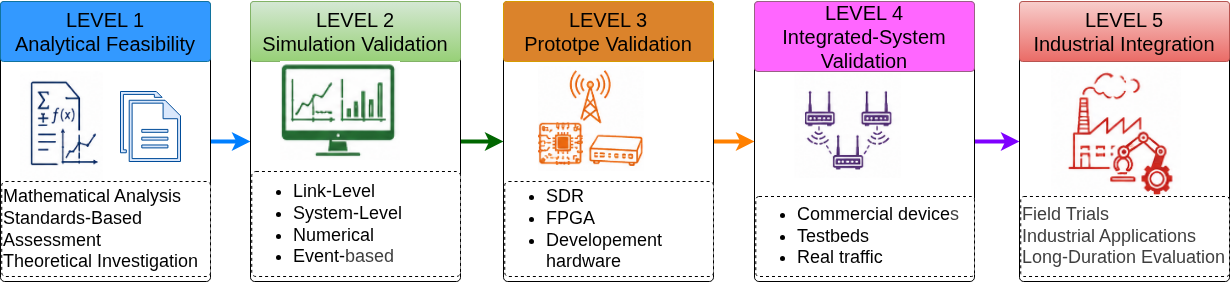
\includegraphics[width=\textwidth]
    {figures/DECT_framework.png}
    \caption{Proposed five-level experimental-maturity framework for
    \gls{dectnr} research, progressing from analytical feasibility to
    industrial integration.}
    \label{fig:experimental_maturity}
\end{figure*}

The framework distinguishes five complementary levels of validation.
\emph{Analytical feasibility (L1)} establishes theoretical or
model-based evidence that a mechanism, architecture, or performance
target is technically plausible. \emph{Simulation validation (L2)}
evaluates the proposed mechanism under controlled link-level,
system-level, numerical, or event-based conditions and enables
investigation of scenarios that may be difficult to reproduce
physically. \emph{Prototype validation (L3)} introduces physical
implementation through \gls{sdr}, \gls{fpga}, development hardware,
or over-the-air experiments, thereby exposing implementation-dependent
effects that are typically abstracted in simulation.
\emph{Integrated-system validation (L4)} evaluates mechanisms using
commercial devices or representative testbeds with real protocol
stacks and traffic, providing evidence of their behavior as part of a
complete communication system. Finally, \emph{industrial integration
(L5)} represents validation through field trials, industrial
applications, or long-duration operation under realistic deployment
conditions.

These levels should not be interpreted as a mandatory linear
development path or as a ranking of research quality. Analytical and
simulation-based studies remain essential for theoretical
understanding, controlled experimentation, scalability analysis, and
exploration of scenarios that may be impractical to reproduce in
hardware. Likewise, individual studies may provide evidence at
multiple maturity levels. Rather, progression toward higher levels
indicates increasing exposure to implementation-, integration-, and
deployment-dependent behavior that cannot be represented completely
at lower levels.

The framework is therefore applied to individual technical areas
rather than assigning a single maturity level to \gls{dectnr} as a
whole. Based on the evidence summarized in
Table~\ref{tab:maturity_matrix}, \gls{phy} research shows the strongest
progression toward Levels~3--5, with substantial prototype,
commercial-device/testbed, and field/industrial evidence. Energy
research also exhibits comparatively strong hardware maturity despite
its smaller publication base. In contrast, \gls{mac} and routing/mesh
research are extensively studied but remain predominantly supported by
analytical and simulation-based evaluation. Scheduling and resource
allocation have only limited higher-level evidence, while
\gls{urllc} and particularly \gls{mmtc} remain strongly
simulation-oriented.

The framework consequently separates \emph{research activity} from
\emph{experimental maturity}. A technical area may contain a large
number of studies while still lacking evidence from large-scale
physical testbeds, integrated systems, or industrial deployments.
Conversely, a smaller research area may exhibit comparatively high
experimental maturity when its findings have been reproduced across
hardware, commercial-device, and field-level evaluations. This
distinction provides a structured basis for identifying where future
\gls{dectnr} research can benefit most from progression toward
large-scale, reproducible, cross-layer, and application-oriented
experimental validation.

\section{Conclusion}
\label{sec:conclusion}

This paper assessed the experimental maturity of \gls{dectnr} through
a systematic mapping of 51 primary studies published between 2020 and
July 2026. The results reveal a clear progression from analytical and
simulation-based investigation toward hardware prototypes,
commercial-device testbeds, field trials, and industrial validation.
However, simulation remains the dominant evaluation methodology, and
evidence from large-scale physical systems, field trials, and
industrial measurements remains limited.

Experimental maturity also differs substantially across technical
areas. \gls{phy} and energy research exhibit comparatively strong
hardware and practical validation, whereas \gls{mac}, routing/mesh,
scheduling and resource allocation, \gls{urllc}, and \gls{mmtc}
remain more dependent on simulation or small-scale experimental
evidence. The analysis further identifies three cross-cutting
challenges: limited experimental scale, insufficient cross-layer and
application-oriented evaluation, and heterogeneous experimental
methodologies that constrain reproducibility and cross-study
comparison.

To characterize these differences, this paper introduced a five-level
experimental-maturity framework spanning analytical feasibility,
simulation validation, prototype validation, integrated-system
validation, and industrial integration. The framework distinguishes
research activity from experimental maturity and provides a structured
basis for assessing how individual technical areas progress toward
practical validation.

Future research should prioritize large-scale multi-device and
multi-hop testbeds, heterogeneous application-oriented traffic,
mobility and interference, long-duration measurements, and
reproducible cross-layer benchmarking. Progress in these areas is
essential for translating the capabilities demonstrated in analytical,
simulation, and small-scale experimental studies into predictable and
dependable \gls{dectnr} performance in real-world \gls{iot} and
industrial deployments.

\bibliographystyle{elsarticle-num}
\bibliography{references}

\end{document}
